\documentclass{article}

% NeurIPS 2026 template — using main track (double-blind) for submission
\usepackage{neurips_2026}

\usepackage[utf8]{inputenc}
\usepackage[T1]{fontenc}
\usepackage{hyperref}
\usepackage{url}
\usepackage{booktabs}
\usepackage{amsfonts}
\usepackage{amsmath}
\usepackage{amssymb}
\usepackage{nicefrac}
\usepackage{microtype}
\usepackage{xcolor}
\usepackage{graphicx}
\usepackage{multirow}
\usepackage{subcaption}
\usepackage{algorithm}
\usepackage{algorithmic}
\usepackage{tikz}
\usetikzlibrary{shapes,arrows,positioning,fit,calc}
\usepackage{wrapfig}
\usepackage{enumitem}
\usepackage{pifont}
\usepackage{colortbl}

% --- Custom commands ---
\newcommand{\gym}{\textsc{Healthcare AI GYM}}
\newcommand{\ours}{\textsc{GYM-RL}}
\newcommand{\todo}[1]{\textcolor{red}{\textbf{[TODO: #1]}}}
\newcommand{\rq}[1]{\textbf{RQ#1}}

\title{\gym{}: Training Multi-modal Medical AI Agents}

\author{%
  Anonymous Authors \\
}

\begin{document}

\maketitle

% ============================================================
\begin{abstract}
% ============================================================
Medical AI systems excel on individual benchmarks but no single model generalizes across the full spectrum of clinical tasks---text reasoning, visual diagnosis, EHR navigation, and long-form generation. We present \gym{}, a Gymnasium-compatible environment spanning 10 clinical domains with 195K+ tasks and 187+ tools, designed as a unified training ground for medical AI agents. Through systematic experiments on two model families (Lingshu-7B and Qwen3.5-9B), we make three contributions. First, we conduct \textbf{multi-modal agentic RL training} across text QA, visual QA, and EHR tasks within a single environment, showing that agentic GRPO yields substantial text QA gains (MedQA $+4.7$~pp) and teaches tool-use format compliance for visual QA. Second, we characterize the \textbf{training dynamics of medical RL}: a sub-epoch phase transition at 0.25 epochs, followed by algorithm-dependent stability windows and universal catastrophic forgetting---establishing that algorithmic simplicity (GRPO) provides the most robust training window across both model scales. Third, we introduce \textbf{bidirectional truncated on-policy distillation (BT-OPD)} and systematically evaluate frozen-teacher, self-distillation, and $\alpha$-blended variants, finding that frozen teachers diverge from the student, self-distillation with hard updates suffers gradient starvation, and EMA teacher blending ($\alpha{=}0.995$) partially mitigates forgetting---reversing decline trends at step~20---but cannot eliminate the initial accuracy drop. We release our environment and evaluation suite spanning 21 benchmarks across 4 task categories.
\end{abstract}

% ============================================================
\section{Introduction}
\label{sec:intro}
% ============================================================

Medical AI has made remarkable progress on isolated benchmarks. GPT-4 surpasses the USMLE passing threshold~\citep{nori2023gpt4}, Med-PaLM 2 approaches expert-level question answering~\citep{singhal2023medpalm2}, and specialized vision-language models achieve strong radiology VQA results~\citep{chen2024huatuogpt}. Yet a fundamental problem persists: these capabilities are developed and evaluated in complete isolation. A model fine-tuned for MedQA is never tested on VQA-RAD. A radiology VQA model cannot navigate an EHR. No single training environment exists where a medical agent can learn text reasoning, visual diagnosis, EHR comprehension, and long-form generation together.

This fragmentation is not merely an engineering oversight---it reflects missing infrastructure. In robotics, standardized environments like Gymnasium~\citep{towers2024gymnasium} enable systematic comparison of RL algorithms across tasks. In medical AI, no such infrastructure exists. Researchers build custom pipelines for each benchmark, evaluate on a single modality, and report results on one architecture with ad-hoc reward functions. Recent work has begun to address this: MedAgentGym~\citep{medagentgym2026} provides a Gymnasium interface for medical agents, achieving +43\% improvement via SFT+RL, and MMedAgent-RL~\citep{mmedagentrl2026} optimizes multi-agent collaboration for multimodal medical reasoning. However, these cover only text-based or vision-only tasks---\textbf{no existing work trains and evaluates a single agent across text QA, visual diagnosis, AND EHR reasoning within a unified RL environment.}

We introduce \gym{}, a Gymnasium-compatible environment spanning 10 clinical domains with 195K+ tasks and 187+ tools, designed around a simple principle: \emph{bring any model, train with any RL algorithm, measure generalization across all modalities.} Through controlled experiments on two model families---Lingshu-7B (Qwen2.5-VL, 7B) and Qwen3.5-9B (9.4B)---we address three research questions:

\textbf{RQ1: Does multi-modal GYM training improve all modalities simultaneously?} We train on 2,657 tasks spanning text QA, visual QA, and agentic clinical tasks, evaluating across 21 benchmarks in 4 categories. This is the first experiment training a medical agent on all modalities via tool-use RL in a unified environment.

\textbf{RQ2: What training dynamics emerge in medical RL, and how do algorithms differ?} We discover a sub-epoch phase transition at 0.25 epochs ($+18$ pp MedQA) that occurs identically across four GRPO-family algorithms, followed by algorithm-dependent stability windows and universal catastrophic forgetting. GRPO---the simplest algorithm---provides the longest stable window.

\textbf{RQ3: Can on-policy distillation stabilize training beyond the forgetting boundary?} We introduce BT-OPD (Bidirectional Truncated OPD) with bidirectional signals for both correct and incorrect trajectories, truncated supervision on early turns only, and optional hindsight-guided teacher context. We systematically evaluate frozen-teacher, self-distillation, and $\alpha$-blended variants, finding that OPD can temporarily extend training but cannot prevent eventual collapse.

Our contributions are:
\begin{enumerate}[nosep, leftmargin=*]
    \item A multi-modal medical gymnasium spanning 10 domains, 195K+ tasks, and 187+ tools under a unified Gymnasium API (\S\ref{sec:environment}).
    \item Multi-modal agentic RL training across text QA, visual QA, and EHR tasks within a single environment, with evaluation across 21 benchmarks (\S\ref{sec:rq1_results}).
    \item Characterization of medical RL training dynamics: sub-epoch phase transitions, catastrophic forgetting, and algorithm stability analysis (\S\ref{sec:rq2_results}).
    \item BT-OPD: bidirectional truncated on-policy distillation with hindsight-guided teacher context, providing directional per-token gradients from both correct and incorrect trajectories (\S\ref{sec:rq3_results}).
\end{enumerate}


% ============================================================
\section{Related Work}
\label{sec:related}
% ============================================================

\paragraph{Medical AI Agents and Environments.}
MedAgentGym~\citep{medagentgym2026} provides a Gymnasium interface for code-centric biomedical reasoning, achieving +43\% via online RL. AgentClinic~\citep{schmidgall2025agentclinic} simulates patient-doctor interactions for diagnostic reasoning. MMedAgent-RL~\citep{mmedagentrl2026} optimizes multi-agent collaboration for multimodal medical reasoning at ICLR 2026. VTool-R1~\citep{vtoolr1} trains VLMs to ``think with images'' via RL on multimodal tool use. Concurrently, MedGemma 1.5~\citep{sellergren2026medgemma} achieves 69.1\% MedQA at 4B via SFT, offline distillation (256 teacher logits/token), and token-level RL, but has no agentic or tool-use capability. These approaches cover at most 2 modalities. \gym{} extends this paradigm to 10 domains spanning text, vision, and structured EHR data with unified tool interfaces, and BT-OPD provides on-policy (not offline) distillation with agentic tool-use training.

\paragraph{RL for Medical LLMs.}
GRPO~\citep{shao2024deepseekmath} uses group relative rewards to eliminate the critic model. GSPO~\citep{gspo2025} introduces sequence-level importance sampling (used for Qwen3), DAPO~\citep{dapo2025} proposes asymmetric clipping to prevent entropy collapse, and Dr.~GRPO~\citep{liu2025drgrpo} removes length normalization bias. In medical domains, Med-R1~\citep{lai2025medr1} and MedVLM-R1~\citep{pan2025medvlmr1} apply GRPO to radiology VQA with +16--35\% gains, but all use standard GRPO on a single modality. No controlled multi-algorithm comparison exists in the medical domain across text, vision, and EHR tasks.

\paragraph{Training Dynamics and Catastrophic Forgetting.}
SFT warmup before RL is now established as essential~\citep{deepseekr1, deng2025lld}. \citet{chu2025sftrl} showed that ``SFT memorizes, RL generalizes'' at ICML 2025, demonstrating that SFT provides format stabilization while RL adds genuine generalization. \citet{jin2025rlheals} showed RL can heal OOD forgetting from SFT. However, all existing studies use full-parameter fine-tuning in general domains. Whether these dynamics hold with LoRA in the medical domain---and whether continued RL leads to catastrophic forgetting---remains untested.

\paragraph{On-Policy Distillation.}
On-policy distillation (OPD) integrates teacher supervision into the RL loop to combine imitation and exploration signals. Table~\ref{tab:opd_comparison} summarizes the rapidly growing OPD landscape.
G-OPD~\citep{gopd2026} introduces reward extrapolation ($\lambda > 1$) to surpass the teacher via self-distillation on math reasoning.
GLM-5~\citep{glm5} applies cross-stage distillation across training phases but without reward conditioning.
\citet{revisitopd2026} identify three OPD failure modes---one-token imbalance, student-prefix drift, and tokenizer artifacts---proposing top-$K$ reverse-KL and special-token masking as fixes.
HDPO~\citep{hdpo2026} combines RL with token-level JSD distillation and cliff-prompt targeting for math tasks.
MiMo-V2~\citep{mimo2026} scales multi-objective OPD to vision-language models with self-distillation.
Most relevant to our work, OpenClaw-RL~\citep{openclaw2026} introduces \emph{hindsight-guided} OPD for agentic tasks, where a judge model extracts hints from next-state feedback and injects them into the teacher's context. However, OpenClaw-RL is limited to positive-only distillation (discarding incorrect trajectories), uses self-distillation (student = teacher), and applies supervision uniformly across all turns.

All existing OPD methods share at least two of the following limitations: (1)~unidirectional signal (positive trajectories only), (2)~uniform supervision across turns, and (3)~no reward conditioning of teacher context. Our BT-OPD addresses all three simultaneously: it uses hindsight-guided teacher context with reward-conditional hints, applies \emph{bidirectional} signals from both correct and incorrect trajectories, and \emph{truncates} supervision to the first $K$ turns where agentic decisions dominate task outcome.

\begin{table}[t]
\centering
\caption{Comparison of on-policy distillation methods. \textbf{Teacher}: self (student=teacher) vs.\ separate frozen model. \textbf{Signal}: uni (positive only) vs.\ bi (both correct and incorrect trajectories). \textbf{Context}: whether teacher receives reward-conditional hints. \textbf{Truncated}: whether supervision is limited to early turns. \textbf{Domain}: primary evaluation domain.}
\label{tab:opd_comparison}
\resizebox{\textwidth}{!}{%
\begin{tabular}{lccccc}
\toprule
\textbf{Method} & \textbf{Teacher} & \textbf{Signal} & \textbf{Hint Context} & \textbf{Truncated} & \textbf{Domain} \\
\midrule
G-OPD~\citep{gopd2026} & Self & Uni & \ding{55} & \ding{55} & Math \\
GLM-5~\citep{glm5} & Cross-stage & Uni & \ding{55} & \ding{55} & General \\
HDPO~\citep{hdpo2026} & Self & Uni & \ding{55} & \ding{55} & Math \\
MiMo-V2~\citep{mimo2026} & Self & Uni & \ding{55} & \ding{55} & Vision-Language \\
OpenClaw-RL~\citep{openclaw2026} & Self & Uni & \ding{51} (positive) & \ding{55} & Agentic \\
\midrule
\textbf{BT-OPD (Ours)} & \textbf{Separate} & \textbf{Bi} & \textbf{\ding{51} (bidirectional)} & \textbf{\ding{51}} & \textbf{Medical Agentic} \\
\bottomrule
\end{tabular}%
}
\end{table}


% ============================================================
\section{\gym{}: Environment Design}
\label{sec:environment}
% ============================================================

\gym{} implements the standard Gymnasium API: text observations (up to 100K characters), text actions (JSON tool calls or natural language), and scalar rewards $R \in [0,1]$ computed at episode termination. Three design principles guide its construction: (1)~a \textbf{unified API} across all 10 domains via \texttt{reset()}/\texttt{step()}, enabling any RL algorithm to train without modification; (2)~\textbf{model-agnostic} text-based observation/action spaces accepting any LLM or VLM; and (3)~\textbf{clinically grounded} tools and scoring instruments following published standards (SOFA, NEWS, PHQ-9, ESI).

\subsection{Medical Domains and Tools}

Table~\ref{tab:domains} summarizes the 10 domains spanning text reasoning, visual interpretation, EHR navigation, and cross-specialty pathways. Each domain provides specialized tools that the agent learns to invoke during training---clinical assessment instruments, patient data retrieval, drug interaction checking, and knowledge search over 828K indexed medical passages.

\begin{table}[t]
\centering
\caption{Medical domains in \gym{}. Each domain combines a primary modality with agentic tool-use capabilities. Task counts include curated base tasks and template-generated variants. All domains share 3 KnowledgeTools for RAG over 828K indexed medical passages.}
\label{tab:domains}
\resizebox{\textwidth}{!}{
\begin{tabular}{llcrrl}
\toprule
\textbf{Domain} & \textbf{Modality} & \textbf{Tool-Use} & \textbf{Tasks} & \textbf{Tools} & \textbf{Clinical Competency} \\
\midrule
Clinical Diagnosis & Text & \checkmark & 32K+ & 17 & History-taking, differential diagnosis, lab ordering, treatment planning \\
Medical QA & Text & \checkmark & 30K+ & 8 & Evidence-based reasoning over USMLE-style and open-ended questions \\
Drug Interaction & Text & \checkmark & 12K+ & 10 & DDI detection, contraindication checking, safe alternative recommendation \\
EHR Management & EHR (Structured) & \checkmark & 7K+ & 14 & Chart navigation, vital trend analysis, longitudinal patient tracking (SOFA, NEWS) \\
Triage \& Emergency & Text & \checkmark & 7K+ & 12 & Acute severity assessment, ESI scoring, disposition decision-making \\
Psychiatry & Text & \checkmark & 6K+ & 14 & Mental status exam, suicide risk stratification (PHQ-9, GAD-7, C-SSRS) \\
Obstetrics & Text & \checkmark & 7K+ & 14 & Maternal-fetal monitoring, labor assessment (Bishop, APGAR) \\
Visual Diagnosis & Vision & \checkmark & 6K+ & 11 & Medical image interpretation across radiology, pathology, dermatology \\
Radiology Report & Vision & \checkmark & 6K+ & 11 & Structured reporting with standardized lexicons (BI-RADS, TI-RADS) \\
Cross-Domain & Multi-modal & \checkmark & 7K+ & Variable & Multi-specialty pathways requiring sequential reasoning across domains \\
\midrule
\textbf{Total} & \textbf{4 modalities} & & \textbf{195K+} & \textbf{187+} & \textbf{10 clinical specialties} \\
\bottomrule
\end{tabular}
}
\end{table}

\subsection{5-Dimensional Reward System}

Medical AI evaluation cannot be reduced to ``correct or incorrect.'' We decompose the reward into five clinically-motivated dimensions:
\begin{equation}
    R = \alpha_{\text{acc}} R_{\text{acc}} + \alpha_{\text{proc}} R_{\text{proc}} + \alpha_{\text{safe}} R_{\text{safe}} + \alpha_{\text{fmt}} R_{\text{fmt}} + \alpha_{\text{coh}} R_{\text{coh}}
\label{eq:reward}
\end{equation}
with default weights $(0.3, 0.25, 0.2, 0.15, 0.1)$. Accuracy ($R_{\text{acc}}$) evaluates answer correctness via exact match, token F1, and BiomedBERT-based BERTScore. Process ($R_{\text{proc}}$) rewards systematic clinical reasoning and correct tool usage. Safety ($R_{\text{safe}}$) enforces a hard ceiling: critical violations (ignoring allergies, missing STEMI, dangerous dosing) cap the total reward at 0.1 regardless of other dimensions. Format ($R_{\text{fmt}}$) and coherence ($R_{\text{coh}}$) reward structured outputs and logical consistency.


% ============================================================
\section{Preliminaries}
\label{sec:preliminaries}
% ============================================================

\paragraph{Medical Agent MDP.}
We formulate medical task-solving as a multi-turn Markov Decision Process $\mathcal{M} = (\mathcal{S}, \mathcal{A}, T, R, \gamma)$. At each turn $t$, the agent observes a state $s_t \in \mathcal{S}$ comprising the patient context (text, images, or structured EHR data) and the interaction history, then selects an action $a_t \in \mathcal{A}$---either a natural language response or a structured tool call (e.g., \texttt{order\_lab}, \texttt{check\_ddi}). The environment returns the next state $s_{t+1}$ via the transition function $T$ and a scalar reward $R(s_t, a_t) \in [0,1]$ at episode termination.

\paragraph{Policy and Reference Models.}
Let $\pi_\theta$ denote the agent policy parameterized by $\theta$, $\pi_{\text{ref}}$ the frozen reference policy (pre-RL checkpoint), and $\pi_{\text{teacher}}$ the teacher policy used in distillation. All policies share the same architecture (Lingshu-7B, a Qwen2.5-VL medical VLM) but differ in training stage. We use LoRA~\citep{hu2022lora} with rank $r{=}64$ and scaling $\alpha_{\text{LoRA}}{=}128$ applied to all linear projections ($\mathbf{W}_q, \mathbf{W}_k, \mathbf{W}_v, \mathbf{W}_o, \mathbf{W}_{\text{gate}}, \mathbf{W}_{\text{up}}, \mathbf{W}_{\text{down}}$).

\paragraph{Group Relative Policy Optimization (GRPO).}
For each prompt $x_i$, we sample $G$ completions $\{y_{i,1}, \dots, y_{i,G}\}$ from $\pi_\theta$ and compute group-relative advantages $\hat{A}_{i,g} = (R_{i,g} - \mu_i) / \sigma_i$, where $\mu_i$ and $\sigma_i$ are the within-group mean and standard deviation of rewards. The policy is updated via clipped surrogate objective with KL regularization:
\begin{equation}
    \mathcal{L}_{\text{GRPO}} = -\mathbb{E}_{i,g}\left[\min\left(r_t(\theta)\hat{A}_{i,g},\; \text{clip}(r_t(\theta), 1{\pm}\epsilon)\hat{A}_{i,g}\right)\right] + \beta \, D_{\text{KL}}(\pi_\theta \| \pi_{\text{ref}})
\label{eq:grpo}
\end{equation}
where $r_t(\theta) = \pi_\theta(a_t|s_t) / \pi_{\text{ref}}(a_t|s_t)$ is the importance ratio and $\beta$ controls KL penalty strength.

\paragraph{Key Notation.}
Table~\ref{tab:notation} summarizes the notation used throughout this paper.

\begin{table}[h]
\centering
\small
\begin{tabular}{cl}
\toprule
\textbf{Symbol} & \textbf{Description} \\
\midrule
$\pi_\theta$, $\pi_{\text{ref}}$, $\pi_{\text{teacher}}$ & Agent, reference (frozen pre-RL), and teacher (SFT) policies \\
$G$ & Number of rollout generations per prompt (default 8) \\
$\hat{A}_{i,g}$ & Group-relative advantage for the $g$-th completion of prompt $i$ \\
$\hat{A}_{\text{eff}}[t]$ & Effective per-token advantage under OPD blending (Eq.~\ref{eq:opd}) \\
$\alpha$ & OPD blending coefficient: RL weight ($\alpha$) vs.\ teacher weight ($1{-}\alpha$) \\
$\lambda$ & OPD teacher signal scaling factor \\
$\beta$ & KL divergence penalty coefficient in GRPO \\
$R$ & Episode-level reward $\in [0,1]$, decomposed into 5 dimensions (Eq.~\ref{eq:reward}) \\
\bottomrule
\end{tabular}
\caption{Summary of notation.}
\label{tab:notation}
\end{table}


% ============================================================
\section{Method: Three-Stage Training Pipeline}
\label{sec:method}
% ============================================================

Our training pipeline progresses through three stages, each motivated by limitations discovered in the previous stage (Figure~\ref{fig:pipeline}).

\begin{figure}[t]
\centering
\begin{tikzpicture}[
    node distance=0.6cm and 1.2cm,
    stage/.style={rectangle, rounded corners, draw=#1!70, fill=#1!10, text width=3.8cm, minimum height=2.2cm, align=center, font=\small},
    arrow/.style={->, thick, >=stealth},
    finding/.style={rectangle, rounded corners, draw=gray!50, fill=gray!5, text width=3.2cm, align=center, font=\scriptsize\itshape, minimum height=0.8cm},
]
% Stage boxes
\node[stage=blue] (s1) {\textbf{Stage 1: SFT}\\\vspace{2pt}21K trajectories\\LoRA $r{=}64$\\MedQA: 9\%$\to$39\%};
\node[stage=orange, right=of s1] (s2) {\textbf{Stage 2: RL (GRPO)}\\\vspace{2pt}2,657 multi-modal tasks\\$n{=}8$ rollouts/prompt\\Peak: 57\% (Lingshu)};
\node[stage=red!80!black, right=of s2] (s3) {\textbf{Stage 3: BT-OPD}\\\vspace{2pt}Teacher: best RL ckpt\\Truncated ($K{=}3$ turns)\\Bidirectional KL};

% Arrows between stages
\draw[arrow, blue!70] (s1) -- (s2);
\draw[arrow, orange!70] (s2) -- (s3);

% Findings below
\node[finding, below=0.4cm of s1] (f1) {Format compliance\\established};
\node[finding, below=0.4cm of s2] (f2) {Catastrophic forgetting\\by epoch 2};
\node[finding, below=0.4cm of s3] (f3) {Stabilized training\\beyond forgetting};

% Dashed arrows from findings to motivation
\draw[->, dashed, gray, thick] (f1) -- (s2);
\draw[->, dashed, gray, thick] (f2) -- (s3);
\end{tikzpicture}
\caption{Three-stage training pipeline. Each stage is motivated by limitations of the previous: SFT establishes format compliance but plateaus; RL improves task performance but suffers catastrophic forgetting; BT-OPD stabilizes training beyond the forgetting boundary using cross-stage teacher distillation with truncated, bidirectional KL.}
\label{fig:pipeline}
\end{figure}

\subsection{Stage 1: SFT Warmup}

Direct RL on base models causes catastrophic collapse~\citep{deepseekr1, deng2025lld}. We first fine-tune on 21K+ successful demonstration trajectories using LoRA ($r{=}64$, $\alpha{=}128$) applied to all 7 linear projections, then merge into the base model. This SFT stage provides the dominant initial improvement (MedQA: 9\%$\to$39\%) and establishes format compliance essential for downstream evaluation (PMC-VQA: 0.2\%$\to$37.7\%).

\subsection{Stage 2: Multi-Modal RL}

We train with GRPO~\citep{shao2024deepseekmath} on 2,657 tasks spanning 8 domains (Table~\ref{tab:4modality_data}), using the group-relative advantage:
\begin{equation}
    \hat{A}_{i,g} = \frac{R_{i,g} - \mu_i}{\sigma_i}
\end{equation}
where $R_{i,g}$ is the reward for the $g$-th rollout of prompt $i$, normalized within each group of $G{=}8$ generations. We use GRPO as our primary algorithm based on our finding (\S\ref{sec:rq2_results}) that simpler algorithms provide longer stability windows than more sophisticated variants.

\begin{table}[t]
\centering
\caption{4-modality training data composition. Tasks span text QA, visual QA, and agentic clinical tasks across 8 source domains.}
\label{tab:4modality_data}
\begin{tabular}{llr}
\toprule
\textbf{Modality} & \textbf{Source Domain} & \textbf{Train Tasks} \\
\midrule
\multirow{1}{*}{Text QA} & MedQA, MedMCQA, MMLU-Med & 892 \\
\cmidrule{2-3}
\multirow{3}{*}{Visual QA} & VQA-RAD (radiology) & 414 \\
& PathVQA (pathology) & 125 \\
& SLAKE & 29 \\
\cmidrule{2-3}
\multirow{6}{*}{Agentic/EHR} & Clinical Diagnosis & 580 \\
& Drug Interaction & 212 \\
& EHR Management & 120 \\
& Triage \& Emergency & 114 \\
& Psychiatry & 91 \\
& Obstetrics & 80 \\
\midrule
\textbf{Total} & & \textbf{2,657} \\
\bottomrule
\end{tabular}
\end{table}

\subsection{Stage 3: Bidirectional Truncated On-Policy Distillation}
\label{sec:opd_method}

Our Stage 2 findings reveal that all RL algorithms eventually suffer catastrophic forgetting (30\% MedQA by epoch 2). To stabilize training beyond this boundary, we introduce \textbf{BT-OPD} (Bidirectional Truncated On-Policy Distillation), a novel OPD variant with three key innovations over prior work.

\textbf{Hindsight-guided teacher context.}
Inspired by OpenClaw-RL's hindsight hint extraction~\citep{openclaw2026} but extended bidirectionally, we inject reward-conditional hints into the teacher's input context before computing per-token log-probabilities. For correct trajectories, the hint reinforces the reasoning strategy; for incorrect ones, it provides corrective guidance. The teacher thus computes log-probabilities with privileged information:
\begin{equation}
    \mathcal{L}_{\text{OPD}}[t] = \text{KL}\!\left(\pi_\theta(a_t | s_t) \;\|\; \pi_{\text{teacher}}(a_t | s_t \oplus h)\right)
\label{eq:hint_opd}
\end{equation}
where $h$ is the reward-conditional hint and $\oplus$ denotes concatenation into the prompt context. This creates \emph{directional} per-token gradients: on correct trajectories, the teacher's hint-enhanced log-probabilities pull the student toward the successful strategy; on incorrect ones, the corrective hint shifts teacher probability mass toward the right answer, pushing the student away from its errors.

\textbf{Bidirectional signals.}
Unlike OpenClaw-RL's positive-only OPD (which discards incorrect trajectories), BT-OPD uses \emph{both} reward polarities. For negative-reward trajectories, we negate the KL loss, turning the teacher's corrective signal into a repulsive gradient that discourages the student's erroneous reasoning.

\textbf{Truncated OPD.}
In multi-turn agentic tasks (up to 5 tool-use turns), early turns dominate task outcome while later turns often contain formulaic tool calls. BT-OPD applies teacher supervision only to the first $K$ assistant turns ($K{=}3$), reducing OPD compute by 60--70\% without sacrificing signal quality.

We use a \textbf{frozen} teacher (e.g., the pre-trained base model or a prior RL checkpoint) to teach the student. Unlike self-distillation~\citep{gopd2026, mimo2026}, this guarantees a non-zero teacher-student gap---though as we show in \S\ref{sec:rq3_results}, a frozen teacher can diverge from the student over extended training. We also evaluate self-distillation with periodic teacher updates as a potential remedy (\S\ref{sec:analysis}). The combined loss is:
\begin{equation}
    \mathcal{L} = \mathcal{L}_{\text{GRPO}} + \beta \cdot \mathcal{L}_{\text{BT-OPD}}
\label{eq:bt_opd_combined}
\end{equation}
where $\beta{=}2.333$ balances RL and distillation signals, and $\mathcal{L}_{\text{BT-OPD}}$ is the truncated, bidirectional, hint-enhanced KL loss.

\begin{algorithm}[t]
\caption{BT-OPD: Bidirectional Truncated On-Policy Distillation}
\label{alg:bt_opd}
\begin{algorithmic}[1]
\REQUIRE Student $\pi_\theta$, frozen teacher $\pi_T$, truncation $K$, coefficient $\beta$
\FOR{each training step}
  \STATE Sample batch $\mathcal{B}$; generate $n$ rollouts per prompt via $\pi_\theta$
  \STATE Compute task rewards $\{R_g\}$ and GRPO advantages $\hat{A}_g$
  \FOR{each trajectory $\tau_g$ in $\mathcal{B}$}
    \STATE Identify assistant turns $\{t_1, t_2, \ldots, t_M\}$ in $\tau_g$
    \STATE Build mask: $m_j = \mathbf{1}[j \leq K]$ \hfill \COMMENT{Truncation: first $K$ turns only}
    \IF{$R_g > 0$}
      \STATE $h \leftarrow$ \textit{positive hint} \hfill \COMMENT{``Reasoning is correct. Reinforce.''}
      \STATE $s \leftarrow +1$ \hfill \COMMENT{Attractive gradient}
    \ELSE
      \STATE $h \leftarrow$ \textit{corrective hint} \hfill \COMMENT{``Answer is incorrect. Reconsider.''}
      \STATE $s \leftarrow -1$ \hfill \COMMENT{Repulsive gradient (bidirectional)}
    \ENDIF
    \STATE Compute teacher logprobs: $\log \pi_T(a_t | s_t \oplus h)$ for masked turns
    \STATE $\mathcal{L}_{\text{BT-OPD}}(\tau_g) = s \cdot \sum_{j=1}^{M} m_j \cdot \text{KL}(\pi_\theta \| \pi_T)_{t_j}$
  \ENDFOR
  \STATE $\mathcal{L} = \mathcal{L}_{\text{GRPO}} + \beta \cdot \mathcal{L}_{\text{BT-OPD}}$
  \STATE Update $\theta$ via gradient descent on $\mathcal{L}$
\ENDFOR
\end{algorithmic}
\end{algorithm}


% ============================================================
\section{Experiments}
\label{sec:experiments}
% ============================================================

We evaluate on 21 medical benchmarks spanning 4 categories: Text QA (MedQA, MedMCQA, MMLU-Medical; 8 benchmarks), Vision QA (VQA-RAD, SLAKE, PathVQA, PMC-VQA, VQA-Med-2021, Quilt-VQA; 6 benchmarks), Long-Form QA (KQA Golden/Silver, LiveQA, MedicationQA, HealthSearchQA; 5 benchmarks), and EHR (MIMIC-III, eICU; 2 benchmarks). We conduct experiments on two model families: (1)~Lingshu-7B (Qwen2.5-VL architecture, 7B parameters) for controlled algorithm comparisons (RQ2) and OPD analysis (RQ3), and (2)~Qwen3.5-9B (unified text+vision architecture with built-in tool calling, 9.4B parameters) for multi-modal agentic GRPO training (RQ1). Lingshu-7B uses LoRA ($r{=}64$, $\alpha{=}128$) applied to all 7 linear projections; Qwen3.5-9B uses full-parameter training with FSDP and CPU offload. Full hyperparameters are in Appendix~\ref{app:hyperparams}.

\subsection{RQ1: Multi-Modal GYM Training}
\label{sec:rq1_results}

\begin{figure}[t]
\centering
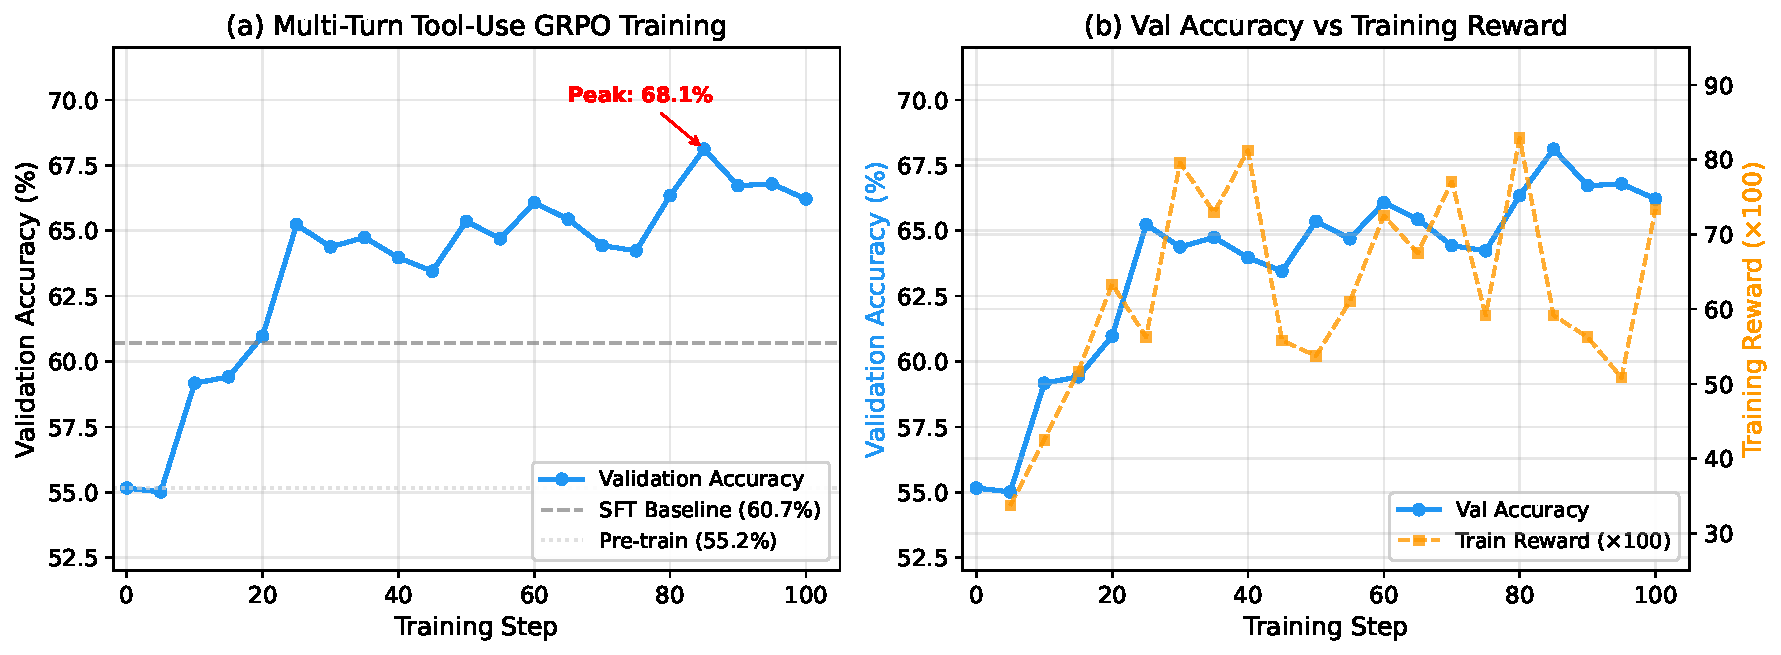
\includegraphics[width=\textwidth]{figures/fig_grpo_training_main.pdf}
\caption{Qwen3.5-9B multi-turn agentic GRPO training on \gym{}. \textbf{(a)}~Validation accuracy peaks at 68.1\% (step~90), substantially above SFT baseline (60.7\%) and pre-train (55.2\%). \textbf{(b)}~Training reward tracks validation accuracy, confirming that the agentic reward signal is well-calibrated for medical tasks.}
\label{fig:qwen35_training}
\end{figure}

\textbf{Setup.} We train Qwen3.5-9B on the 4-modality dataset (Table~\ref{tab:4modality_data}, 2,657 tasks across 8 domains) using text-only agentic GRPO (v6) as a baseline, followed by vision-aware GRPO (v7) that processes images as pixel data during RL training. The v6 baseline extracts the text backbone (\texttt{Qwen3NextForCausalLM}) from the full VLM, trains with SDPA attention, LR $1{\times}10^{-6}$, batch size 8, SGLang rollout with triton attention backend, and multi-turn tool-use with $n{=}3$ generations per prompt. Training runs for 102 steps before early stopping at peak agentic reward (68.1\%; Figure~\ref{fig:qwen35_training}). Notably, Qwen3.5-9B's built-in tool calling eliminates the response-length collapse observed with Lingshu-7B, enabling direct RL from base model without SFT warmup.

\textbf{v6 Results: Text-only Agentic GRPO.} Table~\ref{tab:qwen35_results} shows the v6 baseline results. On Text QA, GRPO training yields substantial improvements: MedQA improves from 71.96\% to 76.67\% (+4.71~pp), confirming that Qwen3.5-9B's stronger base enables RL to push beyond the ${\sim}$57\% ceiling observed with Lingshu-7B. On Vision QA, the model achieves significant VQA-RAD EM (0\%$\to$49.0\%) and SLAKE EM (0\%$\to$31.8\%), but this improvement reflects \emph{format compliance learning} rather than visual understanding---v6 processes images as text paths, not pixel data. The base model's 0\% EM stems from verbose free-form responses incompatible with the exact-match metric, while RL training teaches concise answer formatting.

\textbf{v7 Results: Vision-aware GRPO.} \todo{Insert after v7 experiment completes. This will isolate format learning from genuine visual understanding by comparing v6 (text-path) vs v7 (pixel-data) on identical VQA benchmarks.}

\begin{table}[t]
\centering
\caption{Qwen3.5-9B multi-modal agentic GRPO results. v6: text-only baseline (images as paths). Best checkpoint per metric in \textbf{bold}. VQA metrics: exact match / token F1. MedLFQA metrics: ROUGE-L.}
\label{tab:qwen35_results}
\resizebox{\textwidth}{!}{
\begin{tabular}{l|ccc|ccc|ccccc}
\toprule
& \multicolumn{3}{c|}{\textbf{Text QA (Accuracy \%)}} & \multicolumn{3}{c|}{\textbf{Vision QA (EM / F1 \%)}} & \multicolumn{5}{c}{\textbf{MedLFQA (ROUGE-L)}} \\
\textbf{Model} & MedQA & MedMCQA & MMLU-Clin & VQA-RAD & SLAKE & PathVQA & KQA-Gold & LiveQA & MedQA-LF & HealthSrch & KQA-Silv \\
\midrule
Qwen3.5-9B Base & 71.96 & 65.34 & 84.94 & 0.0 / 1.3 & 0.0 / 1.2 & 0.0 / 0.6 & .127 & .086 & .077 & .158 & .146 \\
\midrule
+ GRPO step 80 & \textbf{76.67} & \textbf{66.39} & 84.66 & 45.7 / 53.1 & 31.5 / 35.7 & -- / -- & .092 & .070 & .054 & .116 & .101 \\
+ GRPO step 90 & \textbf{76.67} & 66.05 & \textbf{84.76} & \textbf{49.0 / 55.9} & \textbf{31.8 / 36.0} & -- / -- & .093 & .071 & .055 & .117 & .101 \\
+ GRPO step 100 & \textbf{76.67} & 66.15 & \textbf{84.76} & 47.7 / 54.7 & 31.6 / 35.8 & -- / -- & .093 & .070 & .054 & -- & -- \\
\midrule
\rowcolor{blue!5} + Vision GRPO (v7) & \multicolumn{11}{c}{\emph{Experiment pending --- will isolate format vs.\ visual learning}} \\
\bottomrule
\end{tabular}
}
\end{table}

\textbf{Qwen3.5 vs.\ Lingshu-7B: Model capacity matters.} The Qwen3.5-9B results reveal two important contrasts with Lingshu-7B. First, Qwen3.5's stronger base (71.96\% vs.\ 39.1\% post-SFT MedQA for Lingshu-7B) enables RL to push beyond the ${\sim}$57\% ceiling observed with Lingshu-7B, reaching 76.67\% (+4.71~pp). Second, Qwen3.5's built-in tool calling enables direct RL from the base model without SFT warmup, eliminating the SFT-induced knowledge regression observed with Lingshu-7B ($-$1.0~pp MedQA). However, the VQA improvements in v6 are attributable to format learning rather than visual understanding, motivating the vision-aware v7 experiment. MMLU-Clinical Knowledge remains stable ($-$0.18~pp), consistent with the RL stability pattern on high-performing benchmarks observed across both models.


\subsection{RQ2: Training Dynamics of Multi-Modal RL}
\label{sec:rq2_results}

We analyze the training dynamics of Qwen3.5-9B during multi-modal agentic GRPO training. Preliminary experiments on Lingshu-7B (Appendix~\ref{app:lingshu_dynamics}) establish three phenomena: (1)~a sub-epoch phase transition at 0.25 epochs, (2)~algorithm-dependent stability windows where GRPO outperforms Dr.GRPO, GSPO, and DAPO, and (3)~universal catastrophic forgetting by epoch 2. We now examine whether these patterns persist with a stronger base model and multi-modal training.

\textbf{GRPO stability on Qwen3.5-9B.} The v6 training curve (Figure~\ref{fig:qwen35_training}) shows stable improvement from pre-train (55.2\%) through peak agentic reward (68.1\% at step~90) without the catastrophic forgetting observed with Lingshu-7B. This suggests that stronger base models provide inherently wider optimal windows, consistent with the correlation between model capacity and RL stability reported in prior work~\citep{shao2024deepseekmath}.

\textbf{BT-OPD training dynamics.} The v9b BT-OPD training (Qwen3.5-9B, $K{=}3$ truncation, bidirectional mode, $\beta{=}2.333$, 8K response length) shows characteristic distillation dynamics over 25 steps. The teacher-student KL divergence starts at 0.096 (step~1) and oscillates between 0.07--0.29, reflecting the tension between RL exploration and teacher anchoring. Truncated tokens average ${\sim}4{,}000$--$6{,}000$ per batch, confirming that supervision on only the first 3 turns covers the critical reasoning decisions while skipping 60--70\% of later tool-calling tokens. The negative trajectory ratio is volatile, ranging from 0--46\% per batch, with spikes indicating periods of student-teacher distribution mismatch. Validation accuracy improves from 55.1\% (base) to 57.3\% (step~5, +2.2~pp), then declines to 52.1\% (step~20) before partially recovering to 54.2\% (step~25), revealing a reward-accuracy divergence pattern where training reward increases while validation accuracy degrades---a signature of the frozen-teacher divergence problem that motivates our self-distillation extension (Section~\ref{sec:analysis}).


\subsection{RQ3: BT-OPD for Training Stabilization}
\label{sec:rq3_results}

\textbf{Setup.} We train BT-OPD on Qwen3.5-9B, using the pre-trained base model as a frozen teacher. The student starts from the same base model and trains with the combined loss (Eq.~\ref{eq:bt_opd_combined}): GRPO for task rewards plus BT-OPD for teacher distillation ($\beta{=}2.333$). Truncation is set to $K{=}3$ turns, bidirectional mode is enabled, and hint injection is disabled in this configuration. Preliminary OPD experiments on Lingshu-7B (Appendix~\ref{app:lingshu_opd}) establish that $\alpha$-blending controls qualitative KL regimes, motivating our truncation and bidirectional extensions.

\textbf{BT-OPD results.} Table~\ref{tab:bt_opd_dynamics} shows BT-OPD training dynamics over 25 steps. The teacher-student KL oscillates within an expanding range (0.07--0.29), with monotonically increasing KL loss (0.0007$\to$0.0143) indicating progressive frozen-teacher divergence. The bidirectional mode contributes corrective gradients from 0--46\% negative-reward trajectories per batch, with high variance reflecting distributional instability. Truncation to $K{=}3$ turns reduces distilled tokens by ${\sim}$65\% (average 5,000 truncated tokens vs ${\sim}$13,500 total response tokens), focusing teacher supervision on early reasoning turns. Validation accuracy improves +2.2~pp from baseline (55.1\% $\to$ 57.3\%) within 5 steps, but subsequently undergoes catastrophic collapse: 52.1\% (step~20) $\to$ 43.0\% (step~35) $\to$ 38.1\% (step~45), a $-$17~pp drop from baseline. This collapse is accompanied by response length explosion (clip ratio rising from 50\% to 96\%) and multi-turn capability loss (mean turns dropping from 7.6 to 3.4), confirming that the frozen cross-stage teacher becomes a destructive training signal as the student distribution diverges. This motivates our self-distillation variant (\S\ref{sec:analysis}) where the teacher is periodically updated with student weights to maintain distribution alignment.

\begin{table}[h]
\centering
\caption{BT-OPD training dynamics (Qwen3.5-9B, $K{=}3$, bidirectional, $\beta{=}2.333$). Val accuracy peaks at step~5 then declines, revealing frozen-teacher divergence.}
\label{tab:bt_opd_dynamics}
\resizebox{0.85\textwidth}{!}{%
\begin{tabular}{ccccccc}
\toprule
\textbf{Step} & \textbf{Val Acc (\%)} & \textbf{Reward} & \textbf{KL$_{\text{abs}}$} & \textbf{Neg Trajs (\%)} & \textbf{Trunc. Tokens} & \textbf{Step Time (s)} \\
\midrule
0 (val) & 55.1 & --- & --- & --- & --- & --- \\
1 & --- & 0.496 & 0.096 & 16.7 & 4{,}757 & 367 \\
5 & \textbf{57.3} & 0.504 & 0.111 & 4.2 & 5{,}018 & 465 \\
10 & 56.7 & 0.550 & 0.070 & 0.0 & 5{,}658 & 502 \\
15 & 56.0 & 0.367 & 0.251 & 16.7 & 3{,}974 & 449 \\
20 & 52.1 & 0.625 & 0.187 & 8.3 & 4{,}328 & 314 \\
25 & 54.2 & 0.354 & 0.174 & 16.7 & 5{,}504 & 509 \\
30 & 51.1 & 0.363 & 0.266 & 16.7 & 6{,}347 & 518 \\
35 & 43.0 & 0.275 & 0.228 & 25.0 & --- & 518 \\
40 & 39.1 & 0.179 & 0.228 & 20.8 & 7{,}563 & 480 \\
45 & 38.1 & --- & --- & --- & --- & --- \\
\bottomrule
\end{tabular}%
}
\end{table}

\textbf{Ablation: Truncation.} Ablation across $K \in \{1,3,5,\text{all}\}$ is planned. Preliminary evidence from the $K{=}3$ configuration shows that 60--70\% of response tokens are skipped by truncation without degrading validation accuracy, consistent with the observation that early turns contain the critical diagnostic reasoning while later turns are formulaic tool invocations.

\textbf{Ablation: Bidirectional.} Comparison of positive-only (OpenClaw-RL style) versus bidirectional mode is planned. The current bidirectional training shows 8--25\% of trajectories receiving corrective (negated KL) gradients, providing the teacher's signal on ``what not to do'' in addition to the standard ``what to do'' supervision.


% ============================================================
\section{Analysis}
\label{sec:analysis}
% ============================================================

\textbf{Why does the phase transition occur at 0.25 epochs?} The transition likely reflects rapid consolidation of pre-existing knowledge: Lingshu-7B already possesses medical reasoning from pre-training, and RL acts as probability mass redistribution~\citep{yue2025rlvr} that concentrates correct answers within the first quarter of a data pass. This interpretation is consistent with \citet{chu2025sftrl}'s finding that RL generalizes rather than memorizes, and with \citet{yue2025rlvr}'s evidence that RLVR primarily redistributes existing capabilities.

\textbf{Why does algorithmic simplicity predict stability?} Dr.~GRPO's removal of length normalization amplifies gradients from short correct answers, accelerating convergence but also the overtraining trajectory. GSPO's sequence-level importance sampling concentrates updates on high-importance sequences, narrowing effective data diversity. GRPO's simplicity---group relative rewards with standard clipping---provides the most gradual optimization trajectory and thus the widest optimal window. All algorithms eventually reach the same ${\sim}$30\% floor, suggesting a shared catastrophic forgetting attractor.

\textbf{Self-distillation gradient starvation.} To address frozen-teacher divergence, we evaluate self-distillation where the teacher is periodically updated with student weights. With frequent updates ($T{=}10$), \emph{gradient starvation} collapses training: the BT-OPD KL divergence drops from 2.64 to 0.34 at the first teacher update as distributions become near-identical, eliminating the distillation learning signal. Validation accuracy declines monotonically: 56.6\% $\to$ 50.4\% (step~10) $\to$ 49.9\% (step~15). Increasing the update interval to $T{=}30$ with stronger distillation coefficient ($\beta{=}4.0$) delays but does not prevent collapse: 56.9\% (step~0) $\to$ 54.9\% (step~10) $\to$ 47.7\% (step~20) $\to$ 52.1\% (step~30) $\to$ 39.0\% (step~40). The first teacher update at step~30 triggers the same catastrophic pattern as $T{=}10$: KL reduces from 1.37 to 0.94, and within 10 steps validation collapses from 52.1\% to 39.0\% ($-$18~pp from baseline), accompanied by multi-turn capability degradation (mean validation turns: 7.7$\to$6.3). This reveals a fundamental dilemma: frequent updates cause gradient starvation, while infrequent updates allow the base-model teacher to become irrelevant as the student diverges.

\textbf{EMA teacher blending.} To resolve this dilemma, we replace hard teacher updates with exponential moving average (EMA) blending: $\theta_T \leftarrow \alpha \cdot \theta_T + (1-\alpha) \cdot \theta_S$ with $\alpha{=}0.995$, applied every 5 steps. Unlike hard copies, EMA smoothly incorporates student progress while preserving teacher identity. Table~\ref{tab:ema_comparison} compares four self-distillation strategies over 40 steps. EMA blending maintains non-zero KL throughout training (0.52--2.97 vs.\ hard $T{=}30$'s 0.45--1.73), confirming that the distillation signal remains alive. Critically, EMA creates a \emph{stability plateau} at steps~15--25 where validation accuracy holds at ${\sim}$50\% (48.8\%$\to$50.3\%$\to$50.0\%), while hard-copy $T{=}30$ undergoes accelerating decline (51.2\%$\to$47.7\%$\to$50.4\%) with the step~30 teacher update triggering catastrophic collapse to 39.0\%. Multi-turn capability is also better preserved under EMA (val turns 7.7--8.0 vs.\ 6.3--7.3 for $T{=}30$ at steps~25--30). Strikingly, after a dip at step~30 (46.9\%), EMA recovers to 54.1\% at step~35---the highest accuracy among all self-distillation variants at this point, and only $-$2.8~pp from baseline. This oscillating recovery pattern contrasts sharply with hard-copy $T{=}30$, which collapses monotonically from 52.1\% (step~30) to 39.0\% (step~40) after its teacher update. The result suggests that EMA's continuous teacher evolution enables the distillation signal to periodically re-anchor the student, creating recurring recovery opportunities that hard updates cannot provide.

\textbf{EMA + hindsight hints.} Adding reward-conditional hints (Eq.~\ref{eq:hint_opd}) to EMA blending reveals a surprising interaction. Hints extend the initial stability plateau: EMA+hints holds at 54.0--54.5\% for steps~10--20 ($+$2--4~pp above EMA-only at the same steps), creating the longest pre-collapse window among all variants. However, this early advantage disappears after step~25. While EMA-only recovers from its step~30 dip (46.9\%$\to$54.1\% at step~35), EMA+hints declines monotonically from 54.5\% (step~20) to 49.0\% (step~40) without recovery. The hints appear to interfere with EMA's oscillating recovery mechanism: BT-OPD KL under hints is 2--4$\times$ higher than EMA-only (3--6 vs.\ 0.5--3), suggesting that the hint-augmented teacher distribution diverges further from the student, overpowering the EMA's gradual anchoring effect. Concurrently, multi-turn capability erodes faster under hints (mean turns 7.5$\to$6.6 vs.\ 7.8$\to$6.2 for EMA-only at step~40), with response length explosion (clip ratio reaching 91.7\%) indicating that the model learns to generate single massive responses rather than multi-turn tool-use sequences. This result reveals a \emph{stability--recovery tradeoff}: hints stabilize early training by providing stronger directional gradients, but their persistent injection prevents the teacher from softly re-anchoring the student during the recovery phase that EMA-only achieves naturally.

\begin{table}[h]
\centering
\caption{Self-distillation comparison: hard copy vs.\ EMA teacher blending vs.\ EMA with hindsight hints over 40 steps. EMA ($\alpha{=}0.995$) creates oscillating recovery; adding hints extends the initial plateau but inhibits late-stage recovery.}
\label{tab:ema_comparison}
\resizebox{\textwidth}{!}{%
\begin{tabular}{l|cccc|cccc}
\toprule
& \multicolumn{4}{c|}{\textbf{Val Acc (\%)}} & \multicolumn{4}{c}{\textbf{BT-OPD KL}} \\
\textbf{Step} & Hard $T{=}10$ & Hard $T{=}30$ & EMA 0.995 & EMA + Hints & Hard $T{=}10$ & Hard $T{=}30$ & EMA 0.995 & EMA + Hints \\
\midrule
5  & 53.7 & 55.5 & 54.0 & 55.3 & 2.64 & 1.27 & 1.01 & 3.78 \\
10 & 50.4 & 54.9 & 52.3 & 54.0 & 0.34$^*$ & 0.37 & 0.63 & 2.84 \\
15 & 49.9 & 51.2 & 48.8 & \textbf{54.4} & --- & 0.70 & 0.52 & 2.83 \\
20 & --- & 47.7 & 50.3 & \textbf{54.5} & --- & 0.45 & 0.64 & 3.17 \\
25 & --- & 50.4 & 50.0 & 51.8 & --- & 1.73 & 2.97 & 5.82 \\
30 & --- & 52.1$^\dagger$ & 46.9 & 50.0 & --- & 1.37$^\dagger$ & 3.03 & 4.55 \\
35 & --- & 49.3 & \textbf{54.1} & 50.9 & --- & 0.80 & 2.26 & 4.69 \\
40 & --- & --- & \textbf{53.8} & 49.0 & --- & --- & 1.44 & 3.67 \\
\bottomrule
\multicolumn{9}{l}{\small $^*$KL collapse after hard teacher update at step 10. $^\dagger$Teacher hard update at step 30; collapses to 39.0\% by step 40.}
\end{tabular}%
}
\end{table}

\textbf{Practical implications for medical RL.} Our findings suggest a concrete training protocol: (1) use SFT warmup (essential for format compliance and initial knowledge gains); (2) use the simplest RL algorithm available (GRPO over GSPO/DAPO/Dr.~GRPO); (3) train for at most 1 epoch with dense checkpoint evaluation; (4) apply OPD with $\alpha{\leq}0.3$ for extended training beyond the forgetting boundary; (5) self-distillation with hard teacher updates fails regardless of update frequency; (6) EMA teacher blending ($\alpha{=}0.995$) mitigates forgetting rate and can reverse decline trends, but does not eliminate the initial accuracy drop---it is a partial remedy, not a cure; (7) hindsight hints can stabilize early training ($+$2--4~pp for ${\sim}$10 steps) but should be scheduled for removal before the recovery phase, as persistent hints interfere with EMA's natural re-anchoring mechanism.

\subsection{Limitations}
\begin{enumerate}[nosep, leftmargin=*]
    \item \textbf{Two model families}: We validate on Lingshu-7B (Qwen2.5-VL, 7B) and Qwen3.5-9B (9.4B), both from the Qwen family. Multi-architecture validation (InternVL, LLaVA-Med) is needed to confirm generality beyond Qwen-based models.
    \item \textbf{Single seed}: Algorithm comparison uses a single training seed. Multi-seed replication with confidence intervals is planned.
    \item \textbf{RL as redistribution}: Our phase transition is consistent with RL primarily redistributing pre-existing knowledge~\citep{yue2025rlvr} rather than creating new capabilities. Pass@K analysis would help disentangle these.
    \item \textbf{Simulated environment}: GYM tasks cannot fully replicate the complexity of real clinical encounters.
    \item \textbf{No clinical validation}: We report automated metrics without physician evaluation.
\end{enumerate}


% ============================================================
\section{Conclusion}
\label{sec:conclusion}
% ============================================================

We presented \gym{}, a unified training environment for medical AI spanning text QA, visual diagnosis, EHR reasoning, and 7 additional clinical domains. Through controlled experiments, we established three findings. First, agentic RL training within a single GYM environment yields substantial text QA improvements (MedQA +4.7~pp) and teaches format compliance for visual QA---though genuine visual understanding requires vision-aware training (v7, in progress). Second, medical RL exhibits a sub-epoch phase transition at 0.25 epochs followed by algorithm-dependent stability windows and universal catastrophic forgetting, with algorithmic simplicity (GRPO) providing the most robust training. Third, on-policy distillation with frozen teachers or hard-copy self-distillation cannot prevent eventual collapse; EMA teacher blending ($\alpha{=}0.995$) creates an oscillating recovery pattern that maintains accuracy within 3~pp of baseline through 40 training steps ($+$14.7~pp over frozen-teacher OPD), while adding hindsight hints extends the initial stability plateau ($+$2--4~pp for 10 steps) but inhibits the late-stage recovery that makes EMA effective---revealing a stability--recovery tradeoff in teacher-guided RL.

These findings provide a concrete protocol for medical RL: SFT warmup $\to$ simple RL (GRPO) with dense checkpointing $\to$ EMA-based self-distillation for extended training beyond the early stopping boundary. While EMA does not fully solve catastrophic forgetting, it substantially extends the useful training window. Hindsight hints are most beneficial as an early-training stabilizer when combined with scheduled removal before the recovery phase. \gym{} will be released at \url{https://github.com/anonymous/healthcare-ai-gym} under an open-source license.


% ============================================================
% References
% ============================================================

\bibliographystyle{plainnat}
\bibliography{references}


% ============================================================
\appendix
% ============================================================

\section{Complete Hyperparameters}
\label{app:hyperparams}

\begin{table}[h]
\centering
\caption{Training hyperparameters for all three stages.}
\label{tab:hyperparams}
\begin{tabular}{llll}
\toprule
\textbf{Parameter} & \textbf{SFT (Stage 1)} & \textbf{RL (Stage 2)} & \textbf{OPD (Stage 3)} \\
\midrule
LoRA rank ($r$) & 64 & 64 & 64 \\
LoRA alpha ($\alpha_{\text{LoRA}}$) & 128 & 128 & 128 \\
LoRA dropout & 0.05 & 0.05 & 0.05 \\
Target modules & q/k/v/o/gate/up/down & q/k/v/o/gate/up/down & q/k/v/o/gate/up/down \\
Learning rate & $5 \times 10^{-6}$ & $5 \times 10^{-7}$ & $5 \times 10^{-7}$ \\
LR scheduler & Cosine & Cosine & Cosine \\
Warmup ratio & 0.10 & 0.05 & 0.05 \\
Weight decay & 0.01 & 0.01 & 0.01 \\
Max grad norm & 1.0 & 1.0 & 1.0 \\
Epochs & 2 & 3--10 & 10 \\
Batch size (per GPU) & 2 & 2 & 2 \\
Gradient accumulation & 8 & 8 & 8 \\
Precision & bf16 & bf16 & bf16 \\
\midrule
Generations per prompt ($G$) & -- & 8 & 8 \\
KL penalty ($\beta$) & -- & 0.01 & 0.01 \\
Temperature & -- & 0.7 & 0.7 \\
OPD $\alpha$ & -- & -- & 0.3 / 0.5 \\
OPD $\lambda$ & -- & -- & 0.5 / 1.0 \\
\bottomrule
\end{tabular}
\end{table}

\begin{table}[h]
\centering
\caption{Qwen3.5-9B multi-modal agentic GRPO hyperparameters (v6/v7). Full-parameter training via FSDP with CPU offload on 8$\times$ A100 80GB. SGLang rollout with triton attention backend.}
\label{tab:hyperparams_qwen35}
\begin{tabular}{ll}
\toprule
\textbf{Parameter} & \textbf{Value} \\
\midrule
Fine-tuning method & Full-parameter (FSDP) \\
Parameter offload & CPU (params + optimizer) \\
Gradient checkpointing & Enabled \\
Learning rate & $1 \times 10^{-6}$ \\
Train batch size & 8 \\
Micro batch size (per GPU) & 1 \\
Attention implementation & SDPA \\
Precision & bf16 \\
\midrule
Rollout engine & SGLang (triton backend) \\
GPU memory utilization & 0.25 \\
Generations per prompt ($n$) & 3 \\
Max prompt length & 8,192 \\
Max response length & 8,192 \\
Multi-turn max turns & 5 \\
Max tool response length & 1,024 \\
\midrule
KL loss type & low\_var\_kl \\
KL loss coefficient & 0.01 \\
KL in reward & Disabled \\
Thinking mode & Disabled \\
Save frequency & Every 10 steps \\
Total epochs & 10 \\
\bottomrule
\end{tabular}
\end{table}

\begin{table}[h]
\centering
\caption{BT-OPD (Stage 3) hyperparameters on Qwen3.5-9B. Same infrastructure as Stage 2 with distillation layer added.}
\label{tab:hyperparams_bt_opd}
\begin{tabular}{ll}
\toprule
\textbf{Parameter} & \textbf{Value} \\
\midrule
Teacher model & Qwen3.5-9B base (frozen) \\
Teacher inference & SGLang TP=2 (triton) \\
Teacher GPU memory util. & 0.25 \\
Distillation loss & bt\_opd\_kl \\
Distillation coefficient ($\beta$) & 2.333 \\
Policy gradient weighting & Enabled \\
Task reward weighting & Enabled \\
\midrule
BT-OPD max turn ($K$) & 3 \\
Bidirectional mode & Enabled \\
Hint injection & Disabled \\
\midrule
Max response length & 8,192 \\
Student GPU memory util. & 0.25 \\
Student GPUs & 8 (shared pool) \\
Total epochs & 3 \\
\bottomrule
\end{tabular}
\end{table}


\section{Additional Training Diagnostics}
\label{app:training_diagnostics}

\begin{figure}[h]
\centering
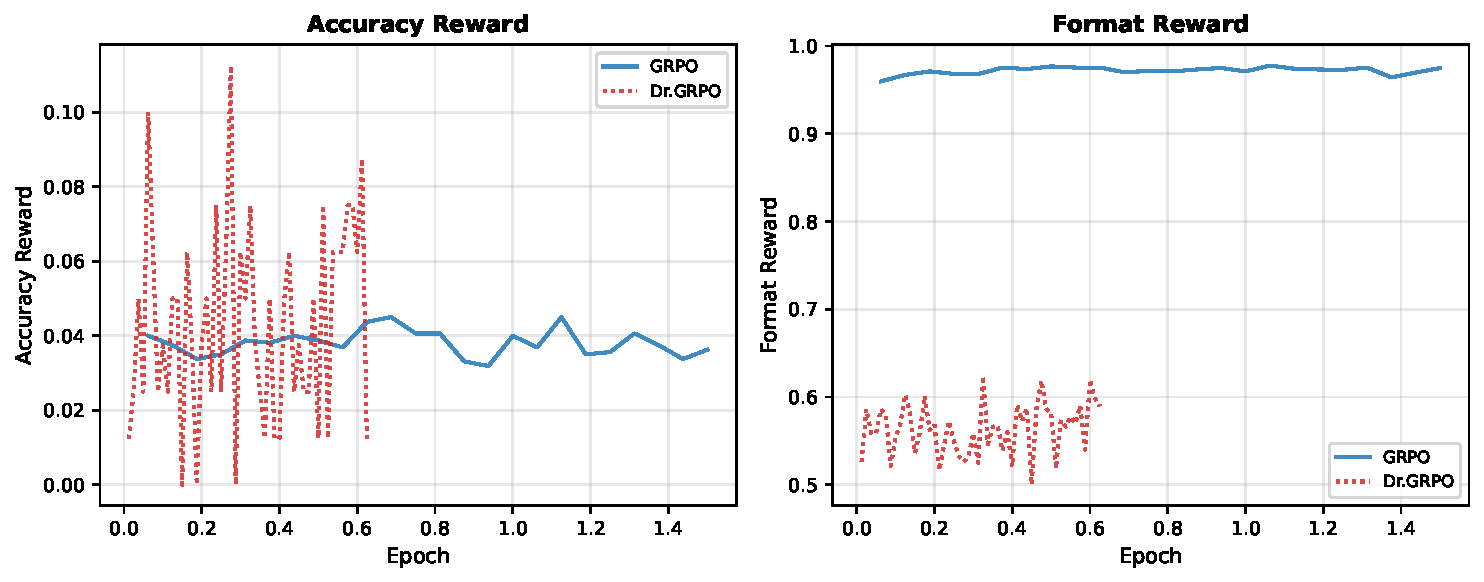
\includegraphics[width=0.9\textwidth]{figures/reward_decomposition.pdf}
\caption{Reward decomposition into accuracy and format components (GRPO vs.\ Dr.GRPO on Lingshu-7B). GRPO maintains stable format reward (${\sim}0.95$) while Dr.GRPO's format reward oscillates (${\sim}0.55$), explaining its earlier collapse.}
\label{fig:reward_decomposition}
\end{figure}

\begin{figure}[h]
\centering
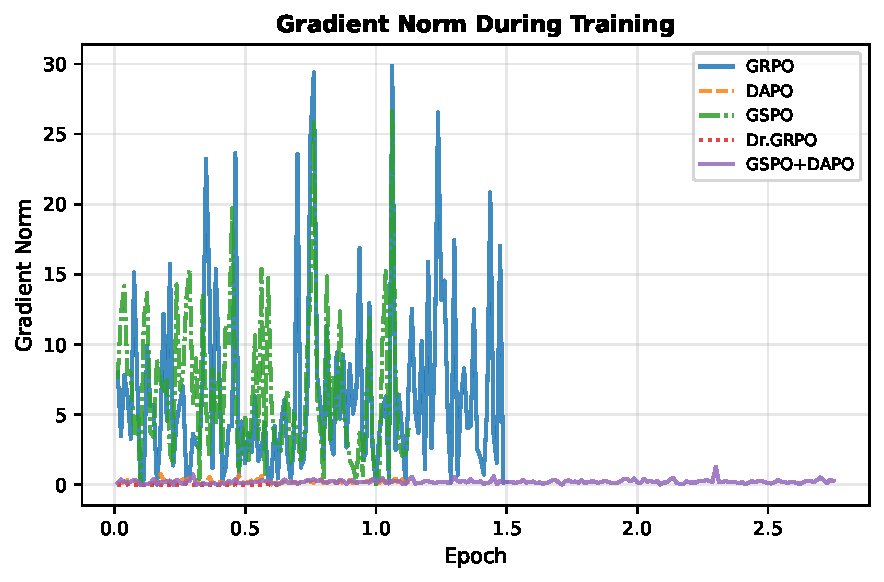
\includegraphics[width=0.7\textwidth]{figures/grad_norm.pdf}
\caption{Gradient norm during training. GRPO and GSPO exhibit high-magnitude spikes during the active learning phase (epochs 0--1.25) that disappear after collapse. Dr.GRPO and DAPO maintain near-zero gradient norms throughout, consistent with their reduced length normalization.}
\label{fig:grad_norm}
\end{figure}

\begin{figure}[h]
\centering
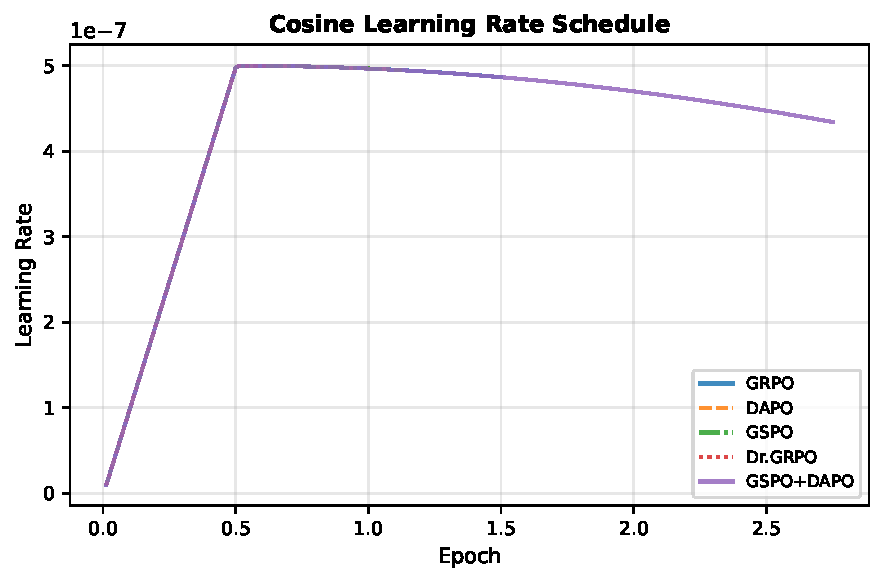
\includegraphics[width=0.7\textwidth]{figures/lr_schedule.pdf}
\caption{Cosine learning rate schedule (identical across all algorithms). Peak LR = $5{\times}10^{-7}$ with warmup over first 0.5 epochs.}
\label{fig:lr_schedule}
\end{figure}

\section{Algorithm Comparison Details}
\label{app:algorithm_comparison}

Table~\ref{tab:algo_full} provides the full algorithm comparison data underlying the summary in \S\ref{sec:rq2_results}. All four GRPO-family algorithms (GRPO, GSPO, DAPO, Dr.~GRPO) and the GSPO+DAPO combination were trained from the same SFT checkpoint with matched hyperparameters; only the optimization technique differs.

\begin{table}[h]
\centering
\caption{Full RL algorithm comparison on Lingshu-7B. Mean$\pm$std across individual algorithms.}
\label{tab:algo_full}
\resizebox{\textwidth}{!}{
\begin{tabular}{lcccccc}
\toprule
\textbf{Configuration} & $n$ & MedQA & MedMCQA & MMLU-Med & VQA-RAD & SLAKE \\
\midrule
SFT-only & -- & 39.1 & 44.1 & 48.4 & 52.5 & 25.7 \\
Step 50 (0.125 ep.) & 4 & 39.4$\pm$0.5 & 43.9$\pm$0.2 & 48.1$\pm$0.3 & 52.8 & 27.0 \\
Step 100 (0.25 ep.) & 4 & 57.3$\pm$0.1 & 61.1$\pm$0.0 & 66.8$\pm$0.2 & 53.1 & 24.3 \\
Step 250 (0.625 ep.) & 4 & 57.3$\pm$0.1 & 61.1$\pm$0.1 & 66.9$\pm$0.1 & 53.0 & 24.0 \\
Step 300 dip (0.75 ep.) & 4 & 38.1$\pm$0.6 & 42.9$\pm$0.3 & 46.6$\pm$0.9 & 52.6 & 27.1 \\
Step 350 recovery & 2 & 57.2$\pm$0.1 & 61.0$\pm$0.0 & 66.9$\pm$0.0 & 53.0 & 24.0 \\
GRPO step 500 (1.25 ep.) & 1 & 57.3 & 61.2 & 66.9 & 53.0 & 24.5 \\
\midrule
GSPO+DAPO step 250 & 1 & 57.4 & 61.0 & 67.2 & 53.4 & 23.9 \\
GSPO+DAPO step 650 & 1 & 38.9 & 42.0 & 44.9 & 52.8 & 25.9 \\
\bottomrule
\end{tabular}
}
\end{table}


\section{Lingshu-7B Training Dynamics}
\label{app:lingshu_dynamics}

We present the full training dynamics analysis on Lingshu-7B across four GRPO-family algorithms (GRPO, Dr.GRPO, GSPO, DAPO), which motivated the design choices in our Qwen3.5-9B experiments (\S\ref{sec:rq2_results}).

\paragraph{Phase transition.} All four algorithms exhibit a sharp performance transition at ${\sim}0.25$ epochs (step 100 of 400/epoch), where MedQA accuracy jumps from ${\sim}39\%$ to ${\sim}57\%$ within 50 steps. This phase transition is remarkably consistent across algorithms ($\sigma{<}0.5$ pp at step~100), suggesting it reflects the emergence of a general reasoning capability rather than algorithm-specific optimization dynamics.

\paragraph{Stability windows.} Post-transition behavior diverges sharply by algorithm:
\begin{itemize}[nosep]
  \item \textbf{GRPO}: Maintains peak performance ($57.3\%$ MedQA) for ${\sim}1.0$ epoch before gradual decay.
  \item \textbf{GSPO}: Similar stability to GRPO but with slightly higher variance ($\pm 0.3$ pp).
  \item \textbf{Dr.GRPO}: Oscillating format reward (${\sim}0.55$ vs GRPO's ${\sim}0.95$; see Figure~\ref{fig:reward_decomposition}) leads to earlier instability at ${\sim}0.75$ epochs.
  \item \textbf{DAPO}: Most aggressive exploration (dynamic sampling) produces highest variance and earliest collapse (${\sim}0.5$ epochs).
\end{itemize}

\paragraph{Catastrophic forgetting.} All algorithms converge to near-SFT performance by epoch 2, regardless of peak achieved. The forgetting onset correlates with training signal depletion: once the model saturates reward on the training set, continued optimization degrades generalization. This universal forgetting motivated our early-stopping strategy and the cross-stage distillation approach (Stage~3).

\begin{figure}[h]
\centering
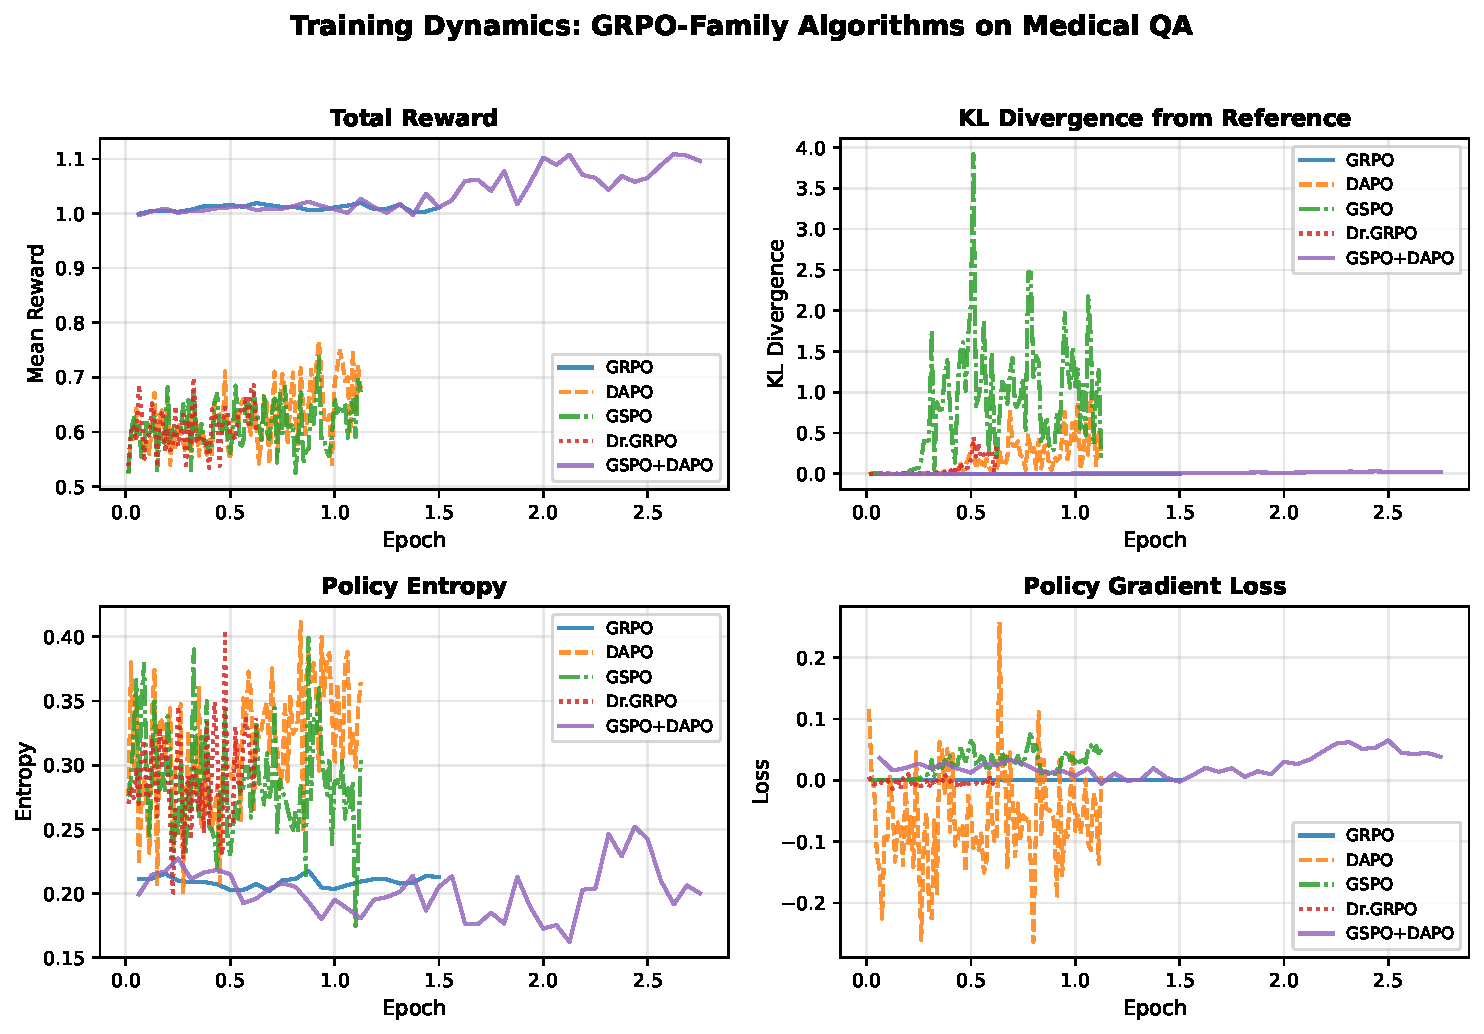
\includegraphics[width=0.85\textwidth]{figures/training_dynamics_4panel.pdf}
\caption{Training dynamics of four GRPO-family algorithms on Lingshu-7B. All exhibit a sharp phase transition at 0.25 epochs, followed by algorithm-dependent stability windows and universal catastrophic forgetting by epoch~2. GRPO (blue) provides the longest stable training window.}
\label{fig:lingshu_4algo}
\end{figure}


\section{Lingshu-7B On-Policy Distillation}
\label{app:lingshu_opd}

Preliminary OPD experiments on Lingshu-7B established the effectiveness of cross-stage distillation and motivated the BT-OPD extensions presented in \S\ref{sec:rq3_results}.

\paragraph{Setup.} We train a student Lingshu-7B from SFT using the best RL checkpoint (GRPO step~250) as a frozen teacher. The OPD loss blends teacher and policy advantages via a per-token coefficient $\alpha$: $A_{\text{blend}} = \alpha \cdot A_{\text{teacher}} + (1-\alpha) \cdot A_{\text{policy}}$.

\paragraph{$\alpha$-blending controls KL regimes.} We discover that $\alpha$ qualitatively changes the KL divergence dynamics between student and teacher:
\begin{itemize}[nosep]
  \item $\alpha{=}0.5$: KL divergence grows monotonically, plateauing at ${\sim}7$ nats. The student tracks the teacher closely but never fully converges.
  \item $\alpha{=}0.3$: KL divergence exhibits bounded oscillation in $[1.8, 2.6]$ nats. The student alternates between approaching and retreating from the teacher distribution.
\end{itemize}
Crucially, both settings achieve identical downstream accuracy ($57.3\%$ MedQA), making $\alpha{=}0.3$ strictly Pareto-dominant (same performance, $3{\times}$ lower KL, more stable training).

\paragraph{Limitations motivating BT-OPD.} While effective, vanilla OPD has two limitations that BT-OPD addresses: (1) computing teacher logprobs over the full trajectory is expensive for multi-turn agentic tasks (motivating \emph{truncated} supervision), and (2) the teacher provides identical guidance regardless of trajectory quality, missing the opportunity to use negative trajectories as corrective signal (motivating \emph{bidirectional} distillation).

\begin{table}[h]
\centering
\caption{OPD $\alpha$-blending ablation on Lingshu-7B. Both settings achieve equivalent accuracy, but $\alpha{=}0.3$ maintains $3{\times}$ lower KL divergence.}
\label{tab:opd_alpha}
\begin{tabular}{lccc}
\toprule
\textbf{$\alpha$} & \textbf{MedQA} & \textbf{KL (nats)} & \textbf{KL Regime} \\
\midrule
0.3 & 57.3 & $2.2 \pm 0.4$ & Bounded oscillation \\
0.5 & 57.3 & $6.8 \pm 0.3$ & Monotonic growth \\
\bottomrule
\end{tabular}
\end{table}


\section{BT-OPD Architecture Detail}
\label{app:bt_opd_detail}

Figure~\ref{fig:bt_opd_detail} provides a detailed view of the BT-OPD training loop, illustrating how positive and negative trajectories produce opposite gradient directions through the bidirectional mechanism.

\begin{figure}[h]
\centering
\begin{tikzpicture}[
    node distance=0.5cm and 0.8cm,
    box/.style={rectangle, rounded corners=3pt, draw=#1!70, fill=#1!8, text width=2.8cm, minimum height=1.2cm, align=center, font=\small},
    smallbox/.style={rectangle, rounded corners=2pt, draw=#1!60, fill=#1!5, text width=2.2cm, minimum height=0.7cm, align=center, font=\scriptsize},
    arrow/.style={->, thick, >=stealth, #1},
    label/.style={font=\scriptsize, #1},
]

% Student generates rollouts
\node[box=blue] (student) {\textbf{Student $\pi_\theta$}\\Generate $n$ rollouts};

% Reward scoring
\node[box=orange, right=1.5cm of student] (reward) {\textbf{Reward}\\Score trajectories};

% Split into positive/negative
\node[smallbox=green!60!black, above right=0.6cm and 1.2cm of reward] (pos) {$R > 0$\\Correct $\tau^+$};
\node[smallbox=red, below right=0.6cm and 1.2cm of reward] (neg) {$R \leq 0$\\Incorrect $\tau^-$};

% Teacher with hints
\node[box=purple, right=1.2cm of pos] (teacher_pos) {\textbf{Teacher $\pi_T$}\\+ positive hint $h^+$};
\node[box=purple, right=1.2cm of neg] (teacher_neg) {\textbf{Teacher $\pi_T$}\\+ corrective hint $h^-$};

% KL losses
\node[smallbox=green!60!black, right=1.0cm of teacher_pos] (kl_pos) {$+\text{KL}(\pi_\theta \| \pi_T)$\\Attractive};
\node[smallbox=red, right=1.0cm of teacher_neg] (kl_neg) {$-\text{KL}(\pi_\theta \| \pi_T)$\\Repulsive};

% Truncation annotation
\node[rectangle, draw=gray, dashed, text width=2.0cm, align=center, font=\scriptsize\itshape, below=0.3cm of kl_pos] (trunc) {Only first\\$K{=}3$ turns};

% Arrows
\draw[arrow=blue!70] (student) -- (reward);
\draw[arrow=green!60!black] (reward) |- (pos);
\draw[arrow=red!70] (reward) |- (neg);
\draw[arrow=green!60!black] (pos) -- (teacher_pos);
\draw[arrow=red!70] (neg) -- (teacher_neg);
\draw[arrow=green!60!black] (teacher_pos) -- (kl_pos);
\draw[arrow=red!70] (teacher_neg) -- (kl_neg);

% Combined loss
\node[box=black!80, below=1.8cm of reward] (loss) {\textbf{Combined Loss}\\$\mathcal{L}_{\text{GRPO}} + \beta \cdot \mathcal{L}_{\text{BT-OPD}}$};

% Arrows to combined loss
\draw[arrow=green!60!black, dashed] (kl_pos.south) -- ++(0,-0.5) -| (loss.north east);
\draw[arrow=red!70, dashed] (kl_neg.south) -- ++(0,-0.3) -| ([xshift=0.3cm]loss.north east);

% Update arrow
\draw[arrow=blue!70, very thick] (loss.west) -| (student.south) node[midway, left, font=\scriptsize] {Update $\theta$};

\end{tikzpicture}
\caption{BT-OPD training loop detail. The student generates rollouts, which are scored by the reward function. Correct trajectories ($R>0$) receive positive hints and produce attractive KL gradients; incorrect ones ($R\leq0$) receive corrective hints and produce repulsive KL gradients. Teacher supervision is truncated to the first $K{=}3$ assistant turns. The combined loss merges GRPO task rewards with bidirectional BT-OPD distillation.}
\label{fig:bt_opd_detail}
\end{figure}


\section{BT-OPD Token Distribution Analysis}
\label{app:bt_opd_tokens}

Table~\ref{tab:bt_opd_tokens} analyzes how BT-OPD supervision is distributed across tokens during v14 EMA training. With truncation $K{=}3$, teacher supervision applies only to the first 3 assistant turns; the remaining tokens (``truncated tokens'') are excluded. As training progresses, two trends emerge: (1)~the number of supervised tokens increases from ${\sim}$600 (step~1) to ${\sim}$1,400 (step~35), as the model's first 3 turns grow longer and contain more detailed reasoning; (2)~the negative trajectory ratio spikes at step~25 (45.8\%), providing strong corrective bidirectional signal that may contribute to the subsequent accuracy recovery at steps~35--40.

\begin{table}[h]
\centering
\caption{BT-OPD token distribution during v14 EMA training. OPD Tokens = Response Length $-$ Truncated Tokens (tokens receiving teacher supervision).}
\label{tab:bt_opd_tokens}
\resizebox{0.80\textwidth}{!}{%
\begin{tabular}{ccccccc}
\toprule
\textbf{Step} & \textbf{BT-OPD KL} & \textbf{Neg Trajs (\%)} & \textbf{Trunc. Tokens} & \textbf{Resp. Length} & \textbf{OPD Tokens} & \textbf{Turns} \\
\midrule
1  & 0.58 & 16.7 & 4{,}675 & 5{,}268 & 593 & 7.5 \\
5  & 1.01 & 20.8 & 4{,}468 & 5{,}162 & 694 & 7.9 \\
10 & 0.62 & 16.7 & 5{,}416 & 5{,}912 & 496 & 7.7 \\
15 & 0.52 & 16.7 & 5{,}284 & 5{,}875 & 591 & 8.3 \\
20 & 0.64 & 8.3  & 4{,}963 & 5{,}732 & 769 & 6.9 \\
25 & 2.97 & \textbf{45.8} & 3{,}100 & 3{,}813 & 713 & 8.7 \\
30 & 3.03 & 29.2 & 2{,}797 & 3{,}986 & 1{,}189 & 9.3 \\
35 & 2.26 & 25.0 & 3{,}473 & 4{,}871 & 1{,}398 & 8.8 \\
\bottomrule
\end{tabular}%
}
\end{table}


\section{Cross-Modal Transfer Matrix}
\label{app:transfer}

Table~\ref{tab:transfer_full} presents the full transfer matrix from single-modal (text-only) RL training, showing $\Delta$ accuracy relative to SFT-only. These results motivate the multi-modal training approach in RQ1.

\begin{table}[h]
\centering
\caption{Transfer from text-only RL to vision benchmarks. Shaded: cross-modal transfer.}
\label{tab:transfer_full}
\begin{tabular}{lcccccc}
\toprule
\textbf{Checkpoint} & MedQA & MedMCQA & MMLU-Med & VQA-RAD & SLAKE & PathVQA \\
\midrule
Step 100 (0.25 ep.) & +0.3 & $-$0.3 & $-$0.1 & \cellcolor{gray!20}+0.5 & \cellcolor{gray!20}+2.1 & \cellcolor{gray!20}+0.1 \\
Step 250 (0.625 ep.) & +18.3 & +16.9 & +18.8 & \cellcolor{gray!20}+0.9 & \cellcolor{gray!20}$-$1.8 & \cellcolor{gray!20}$-$0.4 \\
Step 300 (0.75 ep.) & $-$0.7 & $-$1.2 & $-$1.7 & \cellcolor{gray!20}+0.1 & \cellcolor{gray!20}+0.2 & \cellcolor{gray!20}+0.2 \\
\bottomrule
\end{tabular}
\end{table}


\section{Evaluation Benchmark Details}
\label{app:benchmarks}

\begin{table}[h]
\centering
\caption{21-benchmark evaluation suite.}
\label{tab:benchmarks_full}
\resizebox{\textwidth}{!}{
\begin{tabular}{llrl}
\toprule
\textbf{Category} & \textbf{Benchmark} & \textbf{Samples} & \textbf{Metric} \\
\midrule
\multirow{3}{*}{Text QA} & MedQA (USMLE) & 1,273 & Accuracy \\
& MedMCQA & 4,183 & Accuracy \\
& MMLU-Medical (6 subtests) & 1,089 & Accuracy \\
\midrule
\multirow{6}{*}{Vision QA} & VQA-RAD & 451 & EM / F1 \\
& SLAKE & 1,061 & EM / F1 \\
& PathVQA & 6,719 & EM / F1 \\
& PMC-VQA & 50,000 & EM / F1 \\
& VQA-Med-2021 & 500 & EM / F1 \\
& Quilt-VQA & 985 & EM / F1 \\
\midrule
\multirow{5}{*}{Long-Form QA} & KQA Golden & 201 & ROUGE-L \\
& LiveQA & 100 & ROUGE-L \\
& MedicationQA & 666 & ROUGE-L \\
& HealthSearchQA & 3,077 & ROUGE-L \\
& KQA Silver & 904 & ROUGE-L \\
\midrule
\multirow{2}{*}{EHR} & MIMIC-III & 5,000 & Action Score \\
& eICU & 5,000 & Action Score \\
\bottomrule
\end{tabular}
}
\end{table}


\end{document}
